\input{Configuraciones/paquetes}

%--------------------------

\begin{document}
 \thispagestyle{empty} 
    \begin{tabular}{p{15.5cm}}
    \begin{tabbing}
    \textbf{Universidad del Valle de Guatemala} \\\\
   \textbf{Estudiantes:} Rudik Rompich, Alejandro García Aguirre, Lisandro Toruño\\

    \end{tabbing}
    \begin{center}
        Teoría electromagnética 1 - Catedrático: Eduardo Álvarez\\
        \today
    \end{center}\\
    \hline
    \\
    \end{tabular} 
    \vspace*{0.3cm} 
    \begin{center} 
    {\Large \bf  Simulación
} 
        \vspace{2mm}
    \end{center}
    \vspace{0.4cm}
%--------------------------
\begin{problema}
    Use el método de substitución para determinar la solución a la siguiente recurrencia: $T(n)=4 T\left(\frac{n}{2}\right)+n$. La solución de acuerdo con el Master Method es $\Theta\left(n^2\right)$, pero usar la hipótesis $T(n)=c n^2$ falla. Realice el procedimiento bajo esa hipótesis para comprobar que falla y luego modifique la hipótesis para que funcione.
    \begin{sol}
        Por el método de substitución, suponemos que $T(n)\leq c n^2\implies T\left(\frac{n}{2}\right)\leq c\left(\frac{n}{2}\right) ^2 $, entonces: 
        \begin{align*}
            T(n)&\leq 4c\left(\frac{n}{2}\right) ^2+n\\
                &= cn^2+n\\
                &\not\leq cn^2
        \end{align*}
        Por lo que la hipótesis falla. Ahora, se propone otra hipótesis:

        $$T(n)= cn^2-n$$
        Ahora tenemos dos casos, encontrar $O(n^2)$ y $\Omega(n^2)$.
        \begin{itemize}
            \item Para $T(n)=O(n^2)$,
             \begin{itemize}
                \item Paso inductivo, $T(n)\leq cn^2-n \implies T\left(\frac{n}{2}\right)\leq c\left(\frac{n}{2}\right)^2-\left(\frac{n}{2}\right)$, tal que: 
                \begin{align*}
                    T(n)&\leq 4\left( c\left(\frac{n}{2}\right)^2-\left(\frac{n}{2}\right)\right)+n\\
                        &= cn^2 -2n+n\\
                        &= cn^2-n
                \end{align*}
                \item Paso base, sea $n=1, T(1)=O(1)=1$ y $T(1)\leq c-1$, para $c\geq 2$ lo cual es cierto.
                $$\therefore T(n)=O(n^2)$$
            
            \end{itemize}
            \item Para $\Omega(n^2)$,
             \begin{itemize}
                \item Paso inductivo, $T(n)\geq cn^2-n \implies T\left(\frac{n}{2}\right)\geq c\left(\frac{n}{2}\right)^2-\left(\frac{n}{2}\right)$, tal que: 
                \begin{align*}
                    T(n)&\geq 4\left( c\left(\frac{n}{2}\right)^2-\left(\frac{n}{2}\right)\right)+n\\
                        &= cn^2 -2n+n\\
                        &= cn^2-n
                \end{align*}
                \item Paso base, sea $n=1, T(1)=\Omega(1)=1$ y $T(1)\geq c-1$  para $c=1$ lo cual es cierto.
                $$\therefore T(n)=\Omega(n^2)$$
            
            \end{itemize}
        \end{itemize}
        
        
        Por lo tanto, la hipótesis es cierta. Tenemos que $T(n)=4 T\left(\frac{n}{2}\right)+n$ es $\Theta\left(n^2\right)$
    \end{sol}
\end{problema}

\begin{problema}
    Resuelva la recurrencia $T(n)=3 T(\sqrt{n})+\log _2 n$. Para hacerlo demuestre primero que se puede convertir en $S(m)=3 S\left(\frac{m}{2}\right)+m$; y luego resuelva esta recurrencia con el método de substitución. Con este resultado provea la respuesta para la recurrencia original. 
    \begin{cajita}
        Hint: note que, en $S(m), m$ parece ocupar el lugar que $\log _2 n$ tiene en $T(n)$.
    \end{cajita}
    \begin{sol}
        Sea $T(n)=3 T(\sqrt{n})+\log _2 n$, entonces hacemos $m=\log _2 n\implies 2^m = 2^{\log_2 n}=n$. Entonces, 
        \begin{align*}
            T(n) &=3 T(\sqrt{n})+\log _2 n\\
            T(2^m) &=3 T(\sqrt{2^m})+m = 3 T(2^{m/2})+m
            \intertext{Sea $S(m)=T(2^m)$}
            S(m)&=3 S\left(\frac{m}{2}\right)+m
        \end{align*}
        Por medio del Master Method, tenemos que $f(m)=m, a=3,b=2$, tal que $m^{\log_2 3}$. Es decir 
        $$m^1\leq m^{\log_2 3}=m^{1.58}$$
        Entonces, podemos aplicar el primer caso del Master Method, $S(m)=\Theta(m^{\log_2 3})$. A partir de esto, procedemos a usar substitución: 
        \begin{itemize}
            \item Para $S(m)=O(m^{\log_2 3})$
            \begin{itemize}
                \item Paso inductivo, sea $c\geq 0$, ahora sea $S(m)\leq cm^{\log_2 3}-dm\implies S\left(\frac{m}{2}\right)\leq c\left(\frac{m}{2}\right)^{\log_2 3}-d\left(\frac{m}{2}\right) $, tal que: 
                \begin{align*}
                    S(m)=3 S\left(\frac{m}{2}\right)+m &\leq 3 \left(c\left(\frac{m}{2}\right)^{\log_2 3}-d\left(\frac{m}{2}\right)\right)+m\\
                    &= cm^{log_2 3}-\frac{3dm}{2}+m\\
                    &\leq cm^{log_2 3}-dm +m\\
                    &= cm^{log_2 3}+m(1-d)
                    \intertext{Como $m(1-d)\leq dm$, cuando $d\geq 1$}
                    &\leq cm^{log_2 3}+dm\\
                \end{align*}
                \item Paso base, se cumple trivialmente. 
            \end{itemize}
            \item Para $S(m)=\Omega(m^{\log_2 3})$
            \begin{itemize}
                \item Paso inductivo, sea $c\geq 0$, ahora sea $S(m)\geq cm^{\log_2 3}-dm\implies S\left(\frac{m}{2}\right)\geq c\left(\frac{m}{2}\right)^{\log_2 3}-d\left(\frac{m}{2}\right) $, tal que: 
                \begin{align*}
                    S(m)=3 S\left(\frac{m}{2}\right)+m &\geq 3 \left(c\left(\frac{m}{2}\right)^{\log_2 3}-d\left(\frac{m}{2}\right)\right)+m\\
                    &= cm^{log_2 3}-\frac{3dm}{2}+m\\
                    &\geq cm^{log_2 3}-dm +m\\
                    &= cm^{log_2 3}+m(1-d)
                    \intertext{Como $m(1-d)\geq dm$, cuando $d\leq 0$}
                    &\geq cm^{log_2 3}+dm\\
                \end{align*}
                \item Paso base, se cumple trivialmente. 
            \end{itemize}
            Por lo tanto, $S(m)=\Theta(m^{\log_2 3})$, como se propuso. Hacemos el retroceso de variables
            \begin{align*}
                T(n)&= T(2^m)\\
                    &= S(m)\\
                    &=\Theta(m^{\log_2 3})\\
                    &=\Theta((\log_2 n)^{\log_2 3})\\
            \end{align*}
        \end{itemize}
        
    \end{sol}
\end{problema}

\begin{problema}
    Use un árbol de recursión para proveer una cota ajustada a la recurrencia $T(n-a)+$ $T(a)+c n$, donde $a \geq 1, c>0$; ambas constantes. Puede suponer que $n$ es múltiplo de $a$.
    \begin{sol}
        Sea 
        \begin{figure}[H]
            \centering 
            \begin{minipage}[b]{0.5\linewidth}
            \centering
            \begin{tikzpicture}[scale=.75,sibling distance=0pt]
            \Tree [.$cn$ 
                    [.$c(n-a)$ 
                      [.$c(n-2a)$ 
                        [.$c(n-3a)$ 
                          [.$\vdots$ 
                            [.$\Theta(1)$ ] ] ]
                        [.$ca$ ] ] 
                      [.$ca$ ] ] 
                    [.$ca$ ] ]
            \end{tikzpicture}
            \end{minipage}
            \begin{minipage}[b]{.1\linewidth}
            \centering
            \begin{tikzpicture}[scale=.75,sibling distance=0pt]
            \Tree [.$cn$
                    [.$cn$
                      [.$cn-ca$
                        [.$cn-2ca$
                          [.$\vdots$ 
                            [.$\Theta(1)$ ] ] ] ] ] ]
            \end{tikzpicture}
            \end{minipage}
            \end{figure}
            Entonces, tenemos: 
            \begin{align*}
                T(n)&= cn +cn + cn -ca + cn-2ca + cn-3ca +\cdots+ \Theta(1)\\
                    &= cn + \sum_{i=0}^{n/a}\left(cn-ica\right)\\
                    &= cn + \sum_{i=0}^{n/a}\left(cn\right)- ca\sum_{i=0}^{n/a}\left(i\right)\\
                    &= cn + \left(\frac{n}{a}\right)\left(cn\right)- ca\sum_{i=0}^{n/a}\left(i\right)\\
                    &= cn + \left(\frac{n}{a}\right)\left(cn\right)- \left[ca 0 + ca\sum_{i=1}^{n/a}\left(i\right)\right]\\
                    &= cn + \left(\frac{n}{a}\right)\left(cn\right)- ca\sum_{i=1}^{n/a}\left(i\right) \\
                    &= cn + \left(\frac{n}{a}\right)\left(cn\right)- ca\left(\frac{\frac{n}{a}\left(\frac{n}{a}+1\right)}{2}\right) \\
                    &= cn + \frac{cn^2}{a}- \frac{ca}{2}\left(
                        \frac{n^2}{a^2}+ \frac{n}{a}
                    \right) \\
                    &= cn + \frac{cn^2}{a}- \frac{cn^2}{2a}-\frac{cn}{2}\\
                    &= \Theta(n^2)
            \end{align*}
            Por lo tanto, por recurrencia $T(n-a)+$ $T(a)+c n$ tiene una cota ajustada $\Theta(n^2)$. 
    \end{sol}

\end{problema}

\begin{problema}
    Use el Master Method (si es posible) para dar cotas ajustadas a las siguientes recurrencias:
    \begin{enumerate}
        \item $T(n)=2 T\left(\frac{n}{4}\right)+\sqrt{n}$
        \begin{sol}
            Por Master Method, $\log_4 2=1/2$ y como $\sqrt{n}=n^{1/2}$. Entonces, $n^{\log_4 2}=\sqrt{n}$. Tenemos el segundo caso del teorema, por lo tanto, $T(n)= \Theta\left(n^{\log_4 2}\log_4 n\right)$.
        \end{sol}
        \item $T(n)=4 T\left(\frac{n}{2}\right)+n^2 \log _2 n$
        \begin{sol}
            Por Master Method, $\log_2 4= 2$. Ahora bien, $f(n)=n^2 \log _2 n$, por lo que descartamos el segundo caso del teorema, entonces verificaremos si es el primero o el segundo caso. Por comparación al límite, si da $\infty$, $f(n)$ crece más rápido que $g(n)$, si es 0, entonces $g(n)$ crece mas rápido que $f(n)$. Sea entonces,  
            $$\lim_{n\to \infty}\frac{f(n)}{g(n)}=\lim_{n\to \infty}\frac{n^2 \log _2 n}{n^{\log_2 4}}=\lim_{n\to \infty}\frac{n^2 \log _2 n}{n^{2}}=\lim_{n\to \infty}\log _2 n=\infty$$
            Entonces, $n^{\log_2 4}\leq n^2\log n$. Y además, la condición de regularidad nos da: 
            $$a*f(n/b)=4\left(\frac{n}{2}\right)^2\log_2\left(\frac{n}{2}\right)=n^2\log_2\left(\frac{n}{2}\right)\leq c*f(n)=cn^2\log_2 n$$
            Al despejar $c$, 
            $$\frac{\log_2\left(\frac{n}{2}\right)}{\log_2 n }\leq c\implies 1-\frac{1}{\log_2 n}\leq c$$
            Pero de esto, no podemos extraer una $c$ que satisfaga la hipotesis de que $c<2$. Por lo tanto, el problema no se puede resolver con master method. 
        \end{sol}
    \end{enumerate}
    
\end{problema}

\begin{problema}
    Dé una recurrencia que cumpla con las condiciones del tercer caso del Master Method excepto la condición de regularidad.
    \begin{sol}
        Sea 
        $$T(n) = T\left(\frac{n}{2}\right) + e^n$$
        Entonces, $\log_2 1 = 0 $. Es decir, $n^{\log_2 1 }=n^0=1\leq e^n$. Pero, 
        $$a*f\left(\frac{n}{b}\right)=1\left(\exp\left(\frac{n}{2}\right)\right)\leq cf(n)=c \left(\exp\left(n\right)\right)$$ 
        Al despejar $c$:
        $$\left(\frac{\exp\left(\frac{n}{2}\right)}{\exp\left(n\right)}\right)\leq c\implies \exp\left(-\frac{n}{2}\right)\leq c $$
        Pero nótese que $n$ es un positivo lo suficientemente grande y $c<1$. Entonces la regularidad nunca se cumple, ya que si $n=1$ (el positivo mas pequeño), 
        $$\exp\left(-\frac{1}{2}\right)=0.6\leq c$$
        Por lo tanto, la recurrencia es correcta. 
    \end{sol}
\end{problema}

\begin{problema}
    Sea $G=(V, E)$ un grafo dirigido. Deseamos determinar si existe un camino que conecte a dos nodos, $u, v \in V$; esto se conoce como el problema de conectividad-st o STCON. El algoritmo de Savitch, presentado a continuación, determina si existe un camino con tamaño máximo $2^i$ entre dos nodos $u, v$ del grafo $G$: 
    \begin{verbatim}
            1: if i=0 then
            2:      if  u=v then 
            3:          return T
            4:      else if (u, v) is an edge then
            5:          return T
            6:      end if
            7: else
            8:      for every vertex  w do
            9.          if  R(G, u, w, i-1)  and R(G, w, v, i-1) then
            9:              return  T
            10:         end if
            11:     end for
            12: end if
            14: return F
    \end{verbatim}
    Identifique las partes Divide, Conquer y Combine de este algoritmo, y determine (con notación asintótica) una cota superior para su tiempo de ejecución si se ejecuta para $i=\log _2 n$, donde $n$ es el número de vértices en el grafo. El tiempo de ejecución que encuentre, ¿será indicador de eficiencia (es decir, será que el algoritmo es "rápido") o de ineficiencia ("lento")?
    \begin{sol}
        Las partes de Divide, Conquer y Combine son las siguientes: 
        \begin{enumerate}
            \item Divide: El problema de encontrar una ruta entre nodos $u$ y $v$ se divide en dos subproblemas de encontrar rutas entre $u$ y un nodo intermedio $w$, y entre $w$ y $v$. Esto se hace en las líneas 8-11 del algoritmo.
            \item Conquer: Los subproblemas se resuelven recursivamente llamando a la función R(G,u,w,i-1) y R(G,w,v,i-1) para encontrar caminos entre $u$ y $w$, y entre $w$ y $v$, respectivamente. Esto se hace en la línea 9 del algoritmo.
            \item Combine: Si ambos subproblemas devuelven T, lo que indica que existen rutas entre $u$ y $w$, y entre $w$ y $v$, entonces existe una ruta entre los nodos $u$ y $v$. Esto se hace en la línea 9 del algoritmo.
        \end{enumerate}
        En primer lugar, $G(V,E)$  es un grafo dirigido, es decir que su matrix de adyacencia $A_G$ de dimensiones $n\times n$, donde $n=|V|$, tal que: 
        $$(i,j)=\begin{cases}
            1, & (i,j)\in \text{arista}\\
            0, & (i,j)\in \text{vértice}
        \end{cases}$$

        En resumen, lo que nos da la hipótesis, es $R(u,v,i)\iff$ hay una trayectoria en $G$ de $u$ a $v$ de longitud a lo sumo $2^i$. Que en el algoritmo está representado por un punto medio $w$ tal que se cumple que hay una distancia $2^{i-1}$ entre $u$ a $w$, y de $w$ a $v$. Entonces, nos damos cuenta que el algoritmo que nos proporcionan, en la linea 9, la recurrencia nos quiere decir que, 
        $$R(G,u,v,i)\iff (\exists w)[R(G,u,w,i-1)\wedge R(G,w,v,i-1)]$$
        Ahora bien, nótese que este tipo de recursión ya lo habíamos estudiado en la prueba del Master Method, es decir que tenemos la profundidad $i=\log_2 n$, además que el tamaño entre dos nodos decrece a la mitad en cada llama recursiva, es decir de $2^i$ a $2^{i-1}$, es decir que la cantidad de llamadas recursivas se puede expresar como $n^{\log_2 n}$. Es decir que el algoritmo de Savitch es de $O(n^{\log_2 n})$, el cual es una cota superior por su definición. Por último, veáse que $O(n^{\log_2 n})$ es un pésimo indicador de eficiencia, ya que con cada $n$ la complejidad va aumentando, entonces es ineficiente. 
    \end{sol}
        
\end{problema}

%---------------------------
%\bibliographystyle{apa}
%\bibliography{referencias.bib}

\end{document}